\chapter{Interpolation}

\section{Introduction}

\subsection{Definition}

\begin{example}
    Suppose we are given the following population data
    \begin{table}[H]
        \centering
        \begin{tabular}{r|c|c|c|c|c|c|c|c}
            year           & 1940 & 1950 & 1960 & 1970 & 1980 & 1990 & 2000 & 2010 \\
            \hline
            Population (M) & 132  & 151  & 179  & 203  & 226  & 249  & 281  & 308
        \end{tabular}
    \end{table}
    We mey ask the question: what was the population in 1965? We can use \term{interpolation} to estimate the population in 1985.

    \begin{figure}[H]
        \centering
        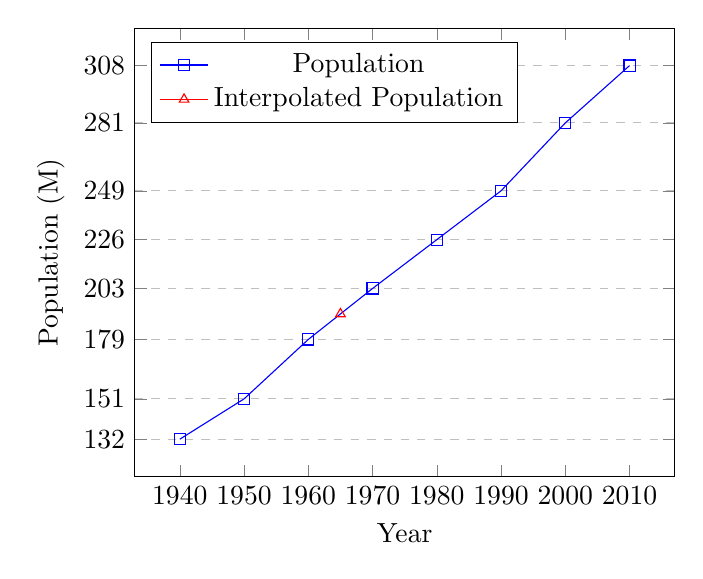
\begin{tikzpicture}
            \begin{axis}[
                    xlabel={Year},
                    ylabel={Population (M)},
                    xtick={1940, 1950, 1960, 1970, 1980, 1990, 2000, 2010},
                    ytick={132, 151, 179, 203, 226, 249, 281, 308},
                    xticklabel style={/pgf/number format/1000 sep=},
                    yticklabel style={/pgf/number format/1000 sep=},
                    legend pos=north west,
                    ymajorgrids=true,
                    grid style=dashed,
                ]

                \addplot[
                    color=blue,
                    mark=square,
                ]
                coordinates {
                        (1940, 132)
                        (1950, 151)
                        (1960, 179)
                        (1970, 203)
                        (1980, 226)
                        (1990, 249)
                        (2000, 281)
                        (2010, 308)
                    };
                \addlegendentry{Population}

                \addplot[
                    color=red,
                    mark=triangle,
                ]
                coordinates {
                        (1965, 191)
                    };
                \addlegendentry{Interpolated Population}

            \end{axis}
        \end{tikzpicture}
        \caption{Population data and interpolated population in 1965}
    \end{figure}

    We may also ask the question: what will the population be in 2020? This will be an \term{extrapolation} problem.
\end{example}

\begin{definition}
    Given a set of \( m \) data points \( \{ (t_i, y_i) \}_{i=1}^{m} \) with \( t_1 < t_2 < \cdots < t_m \), the \textbf{interpolation problem} is to find a function \( g(t) \) from a specific class of functions that \[
        g(t_i) = y_i \quad \text{for all } i = 1, 2, \ldots, m
    \]
\end{definition}

\begin{remark}
    Another use of interpolation is to approximate a function \( f(t) \) by a simpler function \( g(t) \) that is easier to work with.
\end{remark}

\begin{example}
    Suppose we have a function \[
        \operatorname{erf} = \frac{2}{\sqrt{\pi}} \int_{0}^{x} e^{-t^2} \, dt
    \] and we want to approximate it with a polynomial.
    \begin{itemize}
        \item Evaluate \( \operatorname{erf} \) at \( m \) points, \( \{ (x_i, e_i) \}_{i=1}^{m} \)
        \item Interpolate the points with a polynomial \( p(x) \) such that \( p(x_i) = e_i \) for all \( i = 1, 2, \ldots, m \)
        \item Use the interpolant \( p(x) \) in place of \( \operatorname{erf} \)
    \end{itemize}
\end{example}

\subsection{Design Goals for Interpolation}

\begin{enumerate}
    \item Easy to evaluate -- quick, accurate
    \item Gives accurate approximations for \( t \neq t_i \)
    \item Can integrate and differentiate easily
\end{enumerate}

\begin{remark}[Caveats]
    Interpolations come with some caveats.

    \begin{itemize}
        \item Interpolations are not uniques.
        \item Not all interpolations have nice properties
        \item Interpolations does not always give the right solution choice
    \end{itemize}
\end{remark}

\begin{note}
    We assume \textbf{accurate data} has the form \[ \{ (t_i, y_i) \}_{i=1}^m \qquad \text{ or } \qquad \{ t_i, f(t_i) \}_{i=1}^m \] with \[ t_1 < t_2 < \cdots < t_m \]
\end{note}

\subsection{Interpolation Problems}

\begin{example}
    Suppose we want to construct a linear fit for the data \[
        \{ (-1, 2), (1, 1) \}
    \]
    Define \( P_1(t) = b + mt \). We have \( \begin{cases} P_1(-1) = 2 \\ P_1(1) = 1 \end{cases} \implies \begin{cases} b + m (-1) = 2 \\ b + m (1) = 1 \end{cases} \) which yields the solution \[
        b = -\frac{1}{2} \qquad b = \frac{3}{3} \qquad \text{ so } \qquad P_1(t) = \frac{3}{2} - \frac{1}{2}t
    \]
\end{example}

\begin{example}
    Suppose we want to construct a quadratic fit for the data \[
        \{ (-1, 2), (1, 1), (2, 1) \}
    \]
    Define \( P_2(t) = a + bt + ct^2 \). We have \( \begin{cases} P_2(-1) = 2 \\ P_2(1) = 1 \\ P_2(2) = 1 \end{cases} \implies \begin{cases} a + b(-1) + c(-1)^2 = 2 \\ a + b(1) + c(1)^2 = 1 \\ a + b(2) + c(2)^2 = 1 \end{cases} \) which yields \[
        P_2(t) = \frac{4}{3} - \frac{1}{2}t + \frac{1}{6}t^2
    \]
\end{example}

\begin{note}
    We choose polynomial interpolants \[
        P_{m-1}(t) = \sum_{i=1}^m c_i t^{i-1}
    \] because they are easy to evaluate. The operation count is approximately \[
        3n \text{ FLOPs}
    \]
\end{note}

\begin{theorem}[Horner's Rule]
    We can re-write our polynomial as \[
        P_{m-1}(t) = c_1 + t(c_2 + t(c_3 + t(\cdots + t(c_{m-1} + c_m t))))
    \]
\end{theorem}

\begin{note}
    Horner's methods provide some advantages. The operation count reduces to \[
        2m \text{FLOPs}
    \] and it's easier to integrate and differentiate.
\end{note}

\begin{theorem}
    For a set of points \[
        \{ (t_i, y_i) \}_{i=1}^m,
    \] there exists a unique polynomial of degree at less than \( m \) that interpolates the data.
\end{theorem}

\subsubsection{Generalization}

Given a set of points \[
    S = \{ (t_i, y_i) \}_{i=1}^m
\] we find the unique polynomial \[
    P_{m-1}(t) = \sum_{i=1}^{m} c_i t^{i-1}
\] that interpolates the data.